% Created 2024-05-02 木 13:40
% Intended LaTeX compiler: pdflatex
\documentclass[presentation]{beamer}
\usepackage{luatexja}

                 \usepackage{luatexja}
                 \usepackage{luatexja-preset}
\usetheme{Madrid}
\usecolortheme{beetle}
\author{Atsushi Odagiri}
\date{2024-04-25}
\title{パッケージを配ろう}
\hypersetup{
 pdfauthor={Atsushi Odagiri},
 pdftitle={パッケージを配ろう},
 pdfkeywords={},
 pdfsubject={},
 pdfcreator={Emacs 29.2 (Org mode 9.6.12)}, 
 pdflang={English}}
\begin{document}

\maketitle
\begin{frame}{Outline}
\tableofcontents
\end{frame}

\section{パッケージを配ろう}
\label{sec:org7b10f3b}
\begin{frame}[label={sec:org29bed87}]{お前誰よ}
\begin{block}{}
\begin{itemize}
\item Atsushi Odagiri
\item Open Collector
\item Pythonは1.5くらいのころから
\end{itemize}
\end{block}

\begin{block}{}
\begin{center}
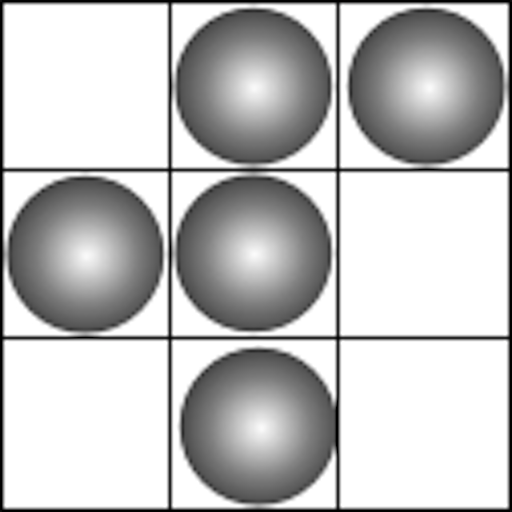
\includegraphics[width=2cm]{./r-penta512.png}
\end{center}

\begin{center}

\includegraphics[width=2cm]{./oc-logo.png}
\end{center}
\begin{center}

\includegraphics[width=2cm]{./logo-w.png}
\end{center}
\end{block}
\end{frame}
\section{パッケージを配るということ}
\label{sec:org81e3064}
\begin{frame}[label={sec:org28309b9}]{パッケージを配るということ}
\begin{itemize}
\item 広く一般に向けて配る
\item 狭い範囲で限られた利用のために配る
\end{itemize}
\end{frame}
\begin{frame}[label={sec:org2c3fc8f},fragile]{広く一般に向けてpypiで配る}
 \begin{itemize}
\item PyPAツールのデフォルト
\item \texttt{tween} でアップロード
\item \texttt{pip} がダウンロードしてインストール
\end{itemize}
\end{frame}
\begin{frame}[label={sec:org11db628}]{狭い範囲で限られた利用のために配る}
\begin{itemize}
\item マイクロサービスのそれぞれて使うようなライブラリ
\end{itemize}
\end{frame}
\section{パッケージを配るためのPEP}
\label{sec:org9e96798}
\begin{frame}[label={sec:org1980494}]{パッケージを配るためのPEP}
\begin{itemize}
\item \href{https://peps.python.org/pep-0458}{PEP 458 – Secure PyPI downloads with signed repository metadata}
\item \href{https://peps.python.org/pep-0480}{PEP 480 – Surviving a Compromise of PyPI: End-to-end signing of packages}
\item \href{https://peps.python.org/pep-0503/}{PEP 503 – Simple Repository API}
\item \href{https://peps.python.org/pep-0592}{PEP 592 – Adding “Yank” Support to the Simple API}
\item \href{https://peps.python.org/pep-0629}{PEP 629 – Versioning PyPI’s Simple API}
\item \href{https://peps.python.org/pep-0658}{PEP 658 – Serve Distribution Metadata in the Simple Repository API}
\item \href{https://peps.python.org/pep-0691}{PEP 691 – JSON-based Simple API for Python Package Indexes}
\item \href{https://peps.python.org/pep-0700}{PEP 700 – Additional Fields for the Simple API for Package Indexes}
\item \href{https://peps.python.org/pep-0714}{PEP 714 – Rename dist-info-metadata in the Simple API}
\end{itemize}
\end{frame}
\begin{frame}[label={sec:org51737c5}]{Simple Repository}
\end{frame}
\begin{frame}[label={sec:orgfbf046e}]{Metadata}
\end{frame}
\begin{frame}[label={sec:orge616ef8}]{JSON}
\end{frame}
\begin{frame}[label={sec:orgdcdf91d}]{PyPIのSimple Repository}
\begin{itemize}
\item \url{https://pypi.org/simple/} とても大きいのでアクセス注意!
\end{itemize}
\end{frame}
\begin{frame}[label={sec:org9b4c287}]{pipでsimple repositoryを使う}
\end{frame}

\section{実践package repository}
\label{sec:org004cfac}
\begin{frame}[label={sec:orgc36659c},fragile]{httplib.server でのお手軽repository}
 \begin{itemize}
\item ダウンロードできるリンクがあればいいので \texttt{http} モジュールでサーバーを起動するだけ
\item wheelファイルのあるディレクトリで実行
\end{itemize}

\begin{verbatim}
python3 -m pip download pyramid
python3 -m http.server
pip install pyramid -f http://localhost:8000/ --no-index
\end{verbatim}

\begin{center}
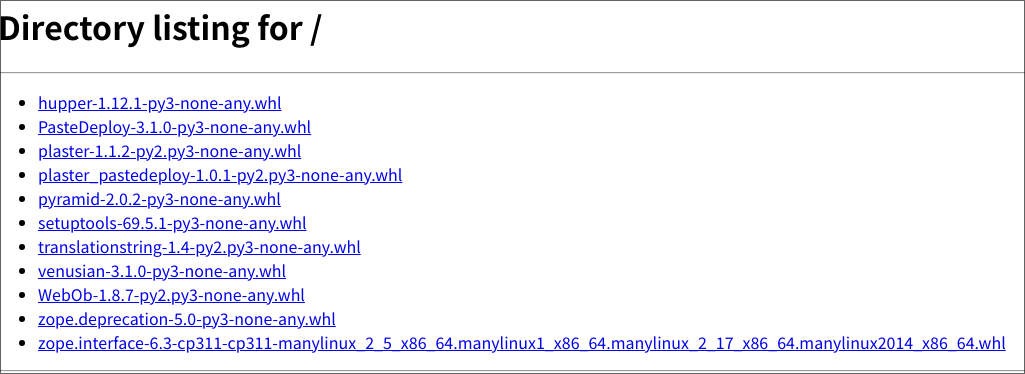
\includegraphics[width=.9\linewidth]{./http-server-simple-repository.png}
\end{center}
\end{frame}

\begin{frame}[label={sec:orgb915b43}]{wsgi app}
\end{frame}
\begin{frame}[label={sec:orgcf2d380}]{metadataを出す}
\end{frame}
\begin{frame}[label={sec:orgb4db4a9}]{jsonに対応}
\begin{itemize}
\item project list
\item project detail
\end{itemize}
\end{frame}
\begin{frame}[label={sec:org5dbba5e}]{The Update Framework}
\begin{itemize}
\item TUF
\end{itemize}
\end{frame}

\section{参考文献}
\label{sec:org61d9b54}
\begin{frame}[label={sec:org21594f8}]{参考文献}
\begin{itemize}
\item PyPA Simple Repository API, \url{https://packaging.python.org/en/latest/specifications/simple-repository-api/}
\item The Update Framework, \url{https://theupdateframework.io/}
\end{itemize}
\end{frame}
\end{document}
